\begin{definition}[\textbf{Triángulo:}]
    Dados tres puntos $\pt{M,N}$ y $\pt{O}$ no colineales, la unión de $\seg{MN}$, $\seg{MO}$, $\seg{NO}$ recibe el nombre de \textit{triángulo} y se denota con $\triangle{MNO}$. Es decir, $\seg{MN} \cup \seg{MO} \cup \seg{NO}$ recibe el nombre de triángulo y se representa $\triangle{OMN}$.

    \begin{figure}[!h]
        \centering
        \begin{tikzpicture}[scale=0.8] 
%\tkzInit[xmax=6,ymax=2, xstep=1]

\tkzDefPoints{% x    y   name
                0  /0   /O,
                2  /4   /N,
                6  /0   /M}

%\tkzDrawPoints(O,M,N)

\tkzLabelPoint[left](O){$\rm{O}$}
\tkzLabelPoint[above](N){$\rm{N}$}
\tkzLabelPoint[right](M){$\rm{M}$}

\tkzDrawPolygon(O,M,N)

\end{tikzpicture}
        \caption{$\triangle{NOM}$}
        \label{fig:triangle}
    \end{figure}
    
\end{definition}

\subsection{Congruencia de Triángulos}

\begin{definition}[\textbf{Triángulos congruentes:}]
    Dos triángulos $\triangle{ABC}$ y $\triangle{PQR}$ son congruentes si sus lados y ángulos correspondientes son congruentes. Simbólicamente $\triangle{ABC} \cong \triangle{PQR}$.

    \begin{figure}[h!]

        \centering

        \begin{subfigure}[b]{.5\textwidth}
            \centering
            \begin{tikzpicture}[scale=0.8]

    % Define los puntos de un triángulo
    \tkzDefPoint(0,0){A}
    \tkzDefPoint(5,0){B}
    \tkzDefPoint(3,3){C}
    
    % Dibuja el triángulo
    \tkzDrawPolygon(A,B,C)

    %\tkzDrawPoints(A,B,C)
    \tkzLabelPoint[left](A){$A$}
    \tkzLabelPoint[right](B){$B$}
    \tkzLabelPoint[above](C){$C$}
    
    % Msrca cada lado con  barras
    \tkzMarkSegment[mark=|](A,B)
    \tkzMarkSegment[mark=||](B,C)
    \tkzMarkSegment[mark=|||](A,C)

    \tkzMarkAngle[arc=l,size=0.8](B,A,C)
    \tkzMarkAngle[arc=ll,size=0.8](C,B,A)
    \tkzMarkAngle[arc=lll,size=0.8](A,C,B)
    
\end{tikzpicture}
            \label{fig:triag-congruence-1}
        \end{subfigure}%
        \begin{subfigure}[b]{.5\textwidth}
            \centering
            \begin{tikzpicture}[scale=0.8,rotate=237]
    
    % Define los puntos de un triángulo.
    \tkzDefPoint(0,0){A}
    \tkzDefPoint(5,0){B}
    \tkzDefPoint(3,3){C}
    
    % Dibuja el triángulo
    \tkzDrawPolygon(A,B,C)

    %\tkzDrawPoints(A,B,C)
    \tkzLabelPoint[above](A){$P$}
    \tkzLabelPoint[left](B){$Q$}
    \tkzLabelPoint[right](C){$R$}
    
    % Marca cada lado con barras.
    \tkzMarkSegment[mark=|](A,B)
    \tkzMarkSegment[mark=||](B,C)
    \tkzMarkSegment[mark=|||](A,C)

    \tkzMarkAngle[arc=l,size=0.8](B,A,C)
    \tkzMarkAngle[arc=ll,size=0.8](C,B,A)
    \tkzMarkAngle[arc=lll,size=0.8](A,C,B)
    
\end{tikzpicture}
            \label{fig:triag-congruence-2}
        \end{subfigure}

        \centering
        \caption{$\triangle{ABC} \cong \triangle{PQR}$}
        \label{fig:triang-congruence}
        
    \end{figure}    
    
\end{definition}

\begin{postulate}[\textbf{Congruencia l-a-l}:]
    Si en un triángulo, dos lados y un ángulo comprendido entre ellos son congruentes con los correspondientes lados y ángulo del segundo triángulo, entonces los dos triángulos son congruentes.

    \begin{figure}[h!]

        \centering

        \begin{subfigure}[b]{.5\textwidth}
            \centering
            \begin{tikzpicture}[scale=0.75]
    
    % Define los puntos del triagnulo
    \tkzDefPoint(0,0){A}
    \tkzDefPoint(5,0){B}
    \tkzDefPoint(-2,3){C}
    
    % Dibuja el triángulo
    \tkzDrawPolygon(A,B,C)
    %\tkzDrawPoints(A,B,C)

    \tkzLabelPoint[left](A){$A$}
    \tkzLabelPoint[above](C){$B$}
    \tkzLabelPoint[right](B){$C$}
    
    % Dibuja ángulo central
    \tkzMarkAngle[size=1cm](B,A,C)
    \tkzLabelAngle[pos=0.5](B,A,C){$\theta$}
    
    % Dibuja las barras en los lados del angulo incluído.
    \tkzMarkSegment[mark=|](A,B)
    \tkzMarkSegment[mark=||](A,C)
\end{tikzpicture}
            \label{fig:congruence-sas1}
        \end{subfigure}%
        \begin{subfigure}[b]{.5\textwidth}
            \centering
            \begin{tikzpicture}[scale=0.75,rotate=203]

    % Define puntos del triángulo
    \tkzDefPoint(0,0){A}
    \tkzDefPoint(5,0){B}
    \tkzDefPoint(-2,3){C}
    
    % Dibuja el triángulo
    \tkzDrawPolygon(A,B,C)
    %\tkzDrawPoints(A,B,C)

    \tkzLabelPoint[above](A){$D$}
    \tkzLabelPoint[right](C){$E$}
    \tkzLabelPoint[left](B){$F$}
    
    % Dibuja ángulo cnetral
    \tkzMarkAngle[size=1cm](B,A,C)
    \tkzLabelAngle[pos=0.5](B,A,C){$\theta$}
    
    % Dibuja las barras en los lados del angulo incluído.
    \tkzMarkSegment[mark=|](A,B)
    \tkzMarkSegment[mark=||](A,C)
\end{tikzpicture}
            \label{fig:congruence-sas2}
        \end{subfigure}

        \centering
        \caption{$\triangle{ABC} \cong \triangle{DEF}$}
        \label{fig:congruencia-sas}
        
    \end{figure}    

\end{postulate}

\clearpage

\begin{postulate}[\textbf{Congruencia a-l-a}:]
    Si en un triángulo, dos ángulos y un lado comprendido entre ellos son congruentes con los correspondientes ángulos y lado del segundo triángulo, entonces los dos triángulos son congruentes.

    \begin{figure}[h!]

        \centering

        \begin{subfigure}[b]{.5\textwidth}
            \centering
            \begin{tikzpicture}[scale=0.8]

    % Define puntos del triángulo
    \tkzDefPoint(0,0){A}
    \tkzDefPoint(5,0){B}
    \tkzDefPoint(1,3){C}
    
    % Dibuja el triángulo
    \tkzDrawPolygon(A,B,C)

    %\tkzDrawPoints(A,B,C)
    \tkzLabelPoint[left](A){$A$}
    \tkzLabelPoint[right](B){$B$}
    \tkzLabelPoint[above](C){$C$}
        
    % Dibuja los ángulos marcados
    \tkzMarkAngle[size=1cm](B,A,C)
    \tkzLabelAngle[pos=0.6](B,A,C){$1$}
    \tkzMarkAngle[size=1.1cm](C,B,A)
    \tkzLabelAngle[pos=0.7](C,B,A){$2$}
    
    % Dibuja las barrita en los lados del ángulo incluído.
    \tkzMarkSegment[mark=|](A,B)
    
    % Rellena la región de los ángulos marcados
    %\tkzFillAngle[fill= gray!40, opacity=.2](B,A,C)
    %\tkzFillAngle[fill= gray!40, opacity=.2](C,B,A)
    
\end{tikzpicture}

            \label{fig:congruence-asa1}
        \end{subfigure}%
        \begin{subfigure}[b]{.5\textwidth}
            \centering
            \begin{tikzpicture}[scale=0.8,rotate=215]
    
    % Define los puntos del triángulo
    \tkzDefPoint(0,0){A}
    \tkzDefPoint(5,0){B}
    \tkzDefPoint(1,3){C}
    
    % Dibuja el triángulo
    \tkzDrawPolygon(A,B,C)

    %\tkzDrawPoints(A,B,C)
    \tkzLabelPoint[above](A){$D$}
    \tkzLabelPoint[left](B){$E$}
    \tkzLabelPoint[right](C){$F$}
        
    % Dibuja los ángulos marcados
    \tkzMarkAngle[size=1cm](B,A,C)
    \tkzLabelAngle[pos=0.6](B,A,C){$1$}
    \tkzMarkAngle[size=1.1cm](C,B,A)
    \tkzLabelAngle[pos=0.7](C,B,A){$2$}
    
    % Dibuja las barritas de del ángulo incluídos
    \tkzMarkSegment[mark=|](A,B)
    
    % Rellena la región de los ángulos marcados.
    %\tkzFillAngle[fill= gray!40, opacity=.2](B,A,C)
    %\tkzFillAngle[fill= gray!40, opacity=.2](C,B,A)
    
\end{tikzpicture}

            \label{fig:congruence-asa2}
        \end{subfigure}

        \centering
        \caption{$\triangle{ABC} \cong \triangle{DEF}$}
        \label{fig:congruencia-asa}
        
    \end{figure}    
    
\end{postulate}

\begin{postulate}[\textbf{Congruencia l-l-l}:]
    Si los tres lados de un triángulo son congruentes con sus correspondientes lados de otro triángulo, entonces los dos triángulos son congruentes.

    \begin{figure}[h!]

        \centering

        \begin{subfigure}[b]{.5\textwidth}
            \centering
            \begin{tikzpicture}[scale=0.8]
    
    % Define los puntos del triángulo
    \tkzDefPoint(0,0){A}
    \tkzDefPoint(5,0){B}
    \tkzDefPoint(3,3){C}
    
    % Dibuja el triángulo
    \tkzDrawPolygon(A,B,C)

    %\tkzDrawPoints(A,B,C)
    \tkzLabelPoint[left](A){$A$}
    \tkzLabelPoint[right](B){$B$}
    \tkzLabelPoint[above](C){$C$}
    
    % Marca cada lado con barritas
    \tkzMarkSegment[mark=|](A,B)
    \tkzMarkSegment[mark=||](B,C)
    \tkzMarkSegment[mark=|||](A,C)
\end{tikzpicture}
            \label{fig:congruence-lll1}
        \end{subfigure}%
        \begin{subfigure}[b]{.5\textwidth}
            \centering
            \begin{tikzpicture}[scale=0.8,rotate=237]
    
    % Define los puntos de un triángulo
    \tkzDefPoint(0,0){A}
    \tkzDefPoint(5,0){B}
    \tkzDefPoint(3,3){C}
    
    % Dibuja el triángulo
    \tkzDrawPolygon(A,B,C)

    %\tkzDrawPoints(A,B,C)
    \tkzLabelPoint[above](A){$D$}
    \tkzLabelPoint[left](B){$E$}
    \tkzLabelPoint[right](C){$F$}
    
    % Marca cada lado con barritas
    \tkzMarkSegment[mark=|](A,B)
    \tkzMarkSegment[mark=||](B,C)
    \tkzMarkSegment[mark=|||](A,C)
\end{tikzpicture}
            \label{fig:congruence-lll2}
        \end{subfigure}

        \centering
        \caption{$\triangle{ABC} \cong \triangle{DEF}$}
        \label{fig:congruencia-lll}
        
    \end{figure}    
    
\end{postulate}

\begin{postulate}[\textbf{Congruencia a-a-l}:]
    Si en un triángulo, dos ángulos y un lado no comprendido entre ellos son congruentes con los correspondientes ángulos y lado del segundo triángulo, entonces los dos triángulos son congruentes.

    \begin{figure}[h!]

        \centering

        \begin{subfigure}[b]{.5\textwidth}
            \centering
            \begin{tikzpicture}[scale=0.8]

    % Define los puntos de un triángulo
    \tkzDefPoint(0,0){A}
    \tkzDefPoint(5,0){B}
    \tkzDefPoint(3,3){C}
    
    % Dibuja el triángulo
    \tkzDrawPolygon(A,B,C)

    %\tkzDrawPoints(A,B,C)
    \tkzLabelPoint[left](A){$A$}
    \tkzLabelPoint[right](B){$B$}
    \tkzLabelPoint[above](C){$C$}
    
    % Dibuja ángulos marcados
    \tkzMarkAngle[size=1cm](B,A,C)
    %\tkzLabelAngle[pos = 0.7](B,A,C){$\alpha$}
    \tkzMarkAngle[size=1cm](C,B,A)
    \tkzMarkAngle[size=1.1cm](C,B,A)
    %\tkzLabelAngle[pos = 0.7](C,B,A){$\beta$}
    
    % Marca los ángulos no incluídos con barritas.
    \tkzMarkSegment[mark=||](A,C)
\end{tikzpicture}
            \label{fig:congruence-aal1}
        \end{subfigure}%
        \begin{subfigure}[b]{.5\textwidth}
            \centering
            \begin{tikzpicture}[xscale=-0.8]
    
    % Define los puntos de un triángulo
    \tkzDefPoint(0,0){A}
    \tkzDefPoint(5,0){B}
    \tkzDefPoint(3,3){C}
    
    % Dibuja el ángulo
    \tkzDrawPolygon(A,B,C)

    %\tkzDrawPoints(A,B,C)
    \tkzLabelPoint[right](A){$D$}
    \tkzLabelPoint[left](B){$E$}
    \tkzLabelPoint[above](C){$F$}
    
    % Dibuja los ángulos marcados
    \tkzMarkAngle[size=1cm](B,A,C)
    %\tkzLabelAngle[pos = 0.7](B,A,C){$\alpha$}
    \tkzMarkAngle[size=1cm](C,B,A)
    \tkzMarkAngle[size=1.1cm](C,B,A)
    %\tkzLabelAngle[pos = 0.7](C,B,A){$\beta$}
    
    % Marca los lados no incluídos con barras
    \tkzMarkSegment[mark=||](A,C)
    
\end{tikzpicture}
            \label{fig:congruence-aal2}
        \end{subfigure}

        \centering
        \caption{$\triangle{ABC} \cong \triangle{DEF}$}
        \label{fig:congruencia-aal}
        
    \end{figure}    
    
\end{postulate}

\clearpage

\begin{postulate}[\textbf{Congruencia hipotenusa-cateto h-c:}]
    Si la hipotenusa y un cateto de un triángulo rectángulo son congruentes con la hipotenusa y el cateto de otro triángulo rectángulo, entonces los triángulos rectángulos son congruentes.

    \begin{figure}[h!]

        \centering

        \begin{subfigure}[b]{.5\textwidth}
            \centering
            \begin{tikzpicture}[scale=0.8]
    
    % Define los puntos de un triángulo
    \tkzDefPoint(0,0){A}
    \tkzDefPoint(4,0){B}
    \tkzDefPoint(0,3){C}
    
    % Dibuja el triángulo
    \tkzDrawPolygon(A,B,C)

    %\tkzDrawPoints(A,B,C)
    \tkzLabelPoint[left](A){$A$}
    \tkzLabelPoint[right](B){$B$}
    \tkzLabelPoint[above](C){$C$}    
    
    % Marca la hipotenusa con barras
    \tkzMarkSegment[mark=||](A,B)
    
    % Marca un lado con barras
    \tkzMarkSegment[mark=|](C,B)
    
    % Marca el ángulo como un ángulo recto.
    \tkzMarkRightAngle(C,A,B)
    
\end{tikzpicture}

            \label{fig:congruence-hlc1}
        \end{subfigure}%
        \begin{subfigure}[b]{.5\textwidth}
            \centering
            \begin{tikzpicture}[xscale=-0.8]
    
    % Define los puntos de un triángulo
    \tkzDefPoint(0,0){A}
    \tkzDefPoint(4,0){B}
    \tkzDefPoint(0,3){C}
    
    % Dibuja un triángulo
    \tkzDrawPolygon(A,B,C)
    %\tkzDrawPoints(A,B,C)
    \tkzLabelPoint[right](A){$A$}
    \tkzLabelPoint[left](B){$B$}
    \tkzLabelPoint[above](C){$C$}        
    
    % Marca la hipotenusa con barras
    \tkzMarkSegment[mark=||](A,B)
    
    % Marca una lado con barras
    \tkzMarkSegment[mark=|](B,C)
    
    % Marca el ángulo como un ángulo recto
    \tkzMarkRightAngle(C,A,B)
\end{tikzpicture}

            \label{fig:congruence-hlc2}
        \end{subfigure}

        \centering
        \caption{$\triangle{ABC} \cong \triangle{DEF}$}
        \label{fig:congruencia-hlc}
        
    \end{figure}    
        
\end{postulate}

\begin{theorem}[\textbf{Congruencia de triángulos isósceles:}]
    Si un triángulo tiene dos lados congruentes (i.e. isósceles), los ángulos opuestos de estos lados son congruentes. Lo opuesto también es verdad.

        \begin{figure}[!h]
            \centering
            \begin{tikzpicture}[scale=0.8]
    % Define the points of the triangle
    \tkzDefPoint(0,0){A}
    \tkzDefPoint(5,0){B}
    \tkzDefPoint(2.5,4){C} % Change the coordinates as needed to make the triangle isosceles
    
    % Draw the triangle
    \tkzDrawPolygon(A,B,C)
    \tkzLabelPoint[left](A){$A$}
    \tkzLabelPoint[right](B){$B$}
    \tkzLabelPoint[above](C){$C$}        
    
    % Mark the equal sides with ticks
    \tkzMarkSegment[mark=||](A,C)
    \tkzMarkSegment[mark=||](B,C)

    % Mark the angles between the base and the sides with ticks
    \tkzMarkAngle[arc=l, size=0.6cm, mark=|](B,A,C)
    \tkzMarkAngle[arc=l, size=0.6cm, mark=|](C,B,A)
\end{tikzpicture}

            \label{fig:isosceles}
            \caption{$\seg{AC} \cong {BC} \leftrightarrow \angle{BAC} \cong \angle{CBA}$}            
        \end{figure}
\end{theorem}

\begin{theorem}[\textbf{Triángulo equilátero es equiángulo:}]
    Un triángulo equilátero es equiángulo. Y un triángulo equiángulo es equilatero. Además, todo triángulo equilátero también es isoscéles.

    \begin{figure}[!h]
        \centering
        \begin{tikzpicture}
    \tkzDefPoint(0,0){A}
    \tkzDefPoint(4,0){B}
    \tkzDefTriangle[equilateral](A,B)
    \tkzGetPoint{C}
    \tkzDrawPolygons(A,B,C)

    \tkzLabelPoint[left](A){$A$}
    \tkzLabelPoint[right](B){$B$}
    \tkzLabelPoint[above](C){$C$}        
  
    \tkzMarkSegments[mark=||](A,B B,C C,A)

  %     % Mark the angles with ticks
    \tkzMarkAngle[arc=l, size=0.5cm, mark=|](B,A,C)
    \tkzMarkAngle[arc=l, size=0.5cm, mark=|](C,B,A)
    \tkzMarkAngle[arc=l, size=0.5cm, mark=|](A,C,B)
    
\end{tikzpicture}


        \label{fig:equilateral}
        \caption{$\seg{AB} \cong {BC}  \cong {AC} \leftrightarrow \angle{BAC} \cong \angle{CBA} \cong \angle{ACB}$}            
    \end{figure}
    
\end{theorem}

\begin{theorem}[\textbf{Separación 1:}]
    Si $O$ está entre $A$ y $B$ en una recta $l$, entonces $O$ y $A$ están del mismo lado de otra recta cualquiera $m$ que contenga a $B$.
\end{theorem}

\begin{theorem}[\textbf{Separación 2:}]
    Si $O$ está entre $B$ y $C$, y $A$ es un punto fuera de $\eline{BC}$, entonces $O$ está en el interior de $\angle{ABC}$.
\end{theorem}

\begin{definition}[\textbf{Bisectriz de un ángulo:}]
    Si $C$ está en el interior de $\angle{ABD}$, y $\angle{ABC} \cong \angle{CBD}$, entonces se dice que $\ray{BC}$ biseca a $\angle{ABD}$ y $\ray{BC}$ se conoce como la bisectriz de $\angle{ABD}$. 

    \begin{figure}[!h]
        \centering
        \begin{tikzpicture}
    % Definir los puntos
    \tkzDefPoint(0,0){A}
    \tkzDefPoint(4,0){B}
    \tkzDefPoint(0,3){D}
    %\tkzDefPointBisector(A,B,C) \tkzGetPoint{D}

    \tkzDefPointBy[rotation=center A angle 45](B)
    \tkzGetPoint{C}

    % Dibujar las lineas y puntos
    \tkzDrawSegment[add=0 and 0.2,-Latex](A,D) 
    \tkzDrawSegment[add=0 and 0.2,-Latex](A,B)

    \tkzDrawSegment[dashed,-Latex,add=0 and 0.2](A,C)
    
    \tkzDrawPoints(A,B,C,D)

    % Etiquetar los puntos
    \tkzLabelPoint[below](A){$B$}
    \tkzLabelPoint[below](B){$D$}
    \tkzLabelPoint[right](D){$A$}
    
    \tkzLabelPoint[right](C){$C$}
    

    % Marcar los ángulos
    \tkzMarkAngle[arc=l,size=0.8,mark=|](B,A,C)
    \tkzMarkAngle[arc=l,size=0.8,mark=|](C,A,D)

\end{tikzpicture}
        \caption{Bizectriz de un ángulo}
        \label{fig:angle-bisector}
    \end{figure}
    
\end{definition}

\begin{theorem}[\textbf{Existencia de una bisectriz}]
    Todo ángulo tiene exactamente una bisectriz.
\end{theorem}

\begin{theorem}[\textbf{Barra transversal}]
    Si $\pt{E}$ está en el interior de $\angle{ABD}$, entonces $\ray{BE}$ interseca $\seg{AD}$.
\end{theorem}